\documentclass[conference, 9pt]{IEEEtran}
\usepackage{amsmath}
\usepackage{amssymb}
\usepackage{color}
\usepackage[font=footnotesize]{subfig}
% \usepackage{eqnarray}
\usepackage{algpseudocode}
\usepackage{varwidth}
\usepackage{paralist}
\usepackage{graphicx}
\usepackage{multirow}
\usepackage{listings}
\usepackage{lipsum}

\graphicspath{{figures/}}

% \renewcommand{\algorithmiccomment}[1]{\hfill\eqparbox{COMMENT}{\# #1}}

\usepackage{url}

% correct bad hyphenation here
\hyphenation{op-tical net-works semi-conduc-tor}


\usepackage{varwidth}
\usepackage{paralist}

% \setlength{\parskip}{1pt}
\setlength{\tabskip}{0em}
% \setlength{\parindent}{1em}
\newcommand{\startcompact}[1]{\par\vspace{-0.75em}\begin{#1}%
\allowdisplaybreaks\ignorespaces}
\newcommand{\stopcompact}[1]{\end{#1}\ignorespaces}

\definecolor{gray20}{gray}{0.20}

\newcommand{\gray}[1]{\color{gray20}{#1}}
\newcommand{\red}[1]{\textcolor{red}{#1}}
\newcommand{\green}[1]{\textcolor{green}{#1}}
\newcommand{\dgreen}[1]{\textcolor{green}{#1}}
\newcommand{\blue}[1]{\textcolor{blue}{#1}}

\begin{document} 

%\title{NoC-based Multi-FPGA Application Mapping:\\ A case study with Boolean Matrix-Vector Multiplication}
% \title{NoC-based Multi-FPGA Application Mapping: A Case Study Accelerating Krylov Sequence Computations over GF(2)}
%\title{Routing packets for multi-FPGA communication: the case of accelerating Krylov sequence computations over GF(2)}
\title{Routing Packets for Multi-FPGA Communication: A Case Study Accelerating Krylov Series Computations over GF(2)}
% \title{Boolean Matrix Vector Multiplication:\\ A Case-study in NoC-based Multi-FPGA Application Mapping}
\maketitle 

\begin{abstract}
Technological advances have enabled FPGA-FPGA communication to assume reliable multi-gigabit data transmission rates. As the consensus grows in the design community and IP vendors towards a standard network-on-chip (NoC) interface, we attempt to explore the benefits of an additional abstraction layer, based on the established framework of NoC, to achieve packetized communication between multiple FPGAs. In particular, we harness existing NoC generator to automatically partition the network across multiple FPGAs and recast the existing design flows of multi-FPGA prototyping and multi-FPGA accelerators based on our automated multi-FPGA NoC partitioning. This is further elucidated by our hardware implementation of boolean matrix vector multiplication, whose scalability is assisted by our ability to partition its underlying network interface over several FPGAs. 
%\lipsum[1]
%\red{TODO: first draft submission after the remarks in RED are all addressed}
%\red{Include \cite{5615563}, \cite{4669212} in related work?}
\end{abstract}


\IEEEpeerreviewmaketitle
\section{Introduction}
The demands on more logic capacity, on-chip dedicated resources, I/O and high-speed transceivers etc., has been rising even as the FPGA application domains grow more pervasive; 
% The resource demands in terms of logic capacity, on-chip resources, I/O resources, and demand for more high-speed transceivers etc., has been rising even as the FPGA application domains grow more pervasive;
and are being met in large part due to Moore scaling. More than Moore scaling too has long been happening at the system level integration via multi-FPGA platforms.
Emulation and verification of large ASICs, and Hardware acceleration, are the two broad application categories where multi-FPGA platforms have been traditionally used.
Today, full system rapid or pre-production prototyping also frequently employs multi-FPGA platforms~\cite{Schelle:2010:INP:1723112.1723116}
\cite{ray2003high}%\footnote{\red{To drop some citations}}
. The design flows involving multi-FPGA systems, often custom designed, present with serious challenges not just in technology integration but a particularly tough one at 
the design automation level. The multi-FPGA partitioning problem is still considered to be one of the toughest challenges in FPGA prototyping/emulation, and is further exasperated
with advanced ASICs consisting of over a billion gates, and particularly time-consuming clustering and partitioning approaches. In practice, the process
is cumbersome and error-prone, requiring manual intervention and knowledge of the partitioned modules.


In addressing the challenges noted in this context, we believe that a design flow mapped over a \emph{standardized} and \emph{simplified} communication framework, such as the 
pervasive packet-switched Network-on-Chip (NoC) framework, together with a automated partitioning step of such a network for multiple FPGAs, could greatly allay the designers of the 
tedious setup phase of multi-FPGA design automation. The partitioned communication network should also be flexible in terms of the choice of topology and router configurations.

% In addressing the challenges noted in this context, we believe that a \emph{standardized} and \emph{simplified} communication framework, such as the 
% pervasive packet-switched Network-on-Chip (NoC) framework, together with an \emph{automated} partitioning scheme targeting multiple FPGAs, could greatly allay the designers of the 
% tedious setup phase of multi-FPGA design automation. The partitioned communication network should also be flexible in terms of topology and router configurations.

% \blue{The partitioned communication network should also be flexible in terms of topology and 
% router configurations. Since several modern day ASICs and MPSoCs also employ NoC interface for communication between modules, our partitioned network would also be 
% effective for prototyping and debugging of these designs on multiple FPGAs, 
% which are otherwise limited by the resource constraints of a single FPGA. This 
% approach is also handy for designing multiple FPGA-based hardware accelerators, 
% using the underlying network as the communication interface.}

With our automated partitioning flow, as a proof-of-concept study, we present the case of hardware acceleration of
boolean matrix vector multiplication occurring in the context of Krylov sequence computations, where the scalability of the communicatin intensive algorithm is 
determined by the ability to partition its network over several FPGAs. Although in incipient stage, our 
approach helps raising the level of abstraction in multi-FPGA design scenario, which has remained an esoteric art of a few hardware designers despite its numerous advantages. 

The remainder of the paper is organized as follows. In the next section, we outline two design flows
which could benefit by our approach. We then present our solution to the multi-FPGA partitioning problem and a discussion of the implementation details
and advantages in Section~\ref{sec:mfpga_part}. In Section~\ref{sec:BMVM} we report a case study of an important algorithm in the context of high-performance computing, along with evaluation results and a discussion. Section~\ref{sec:relwork} discusses some related work, and Section~\ref{sec:conclusion} concludes.


% \section{Introduction}
% FPGAs have been extensively deployed for full system prototyping and 
% verification of large ASIC designs~\cite{gschwind2001fpga, ray2003high}. Lowering costs, as an artifact of advanced 
% manufacturing processes and increasing competition, have rendered FPGA prototyping a considerable advantage over 
% other known alternatives. These include RTL simulation
% %~\cite{geiger1990vlsi}
%  and 
% virtual prototyping,
% %~\cite{valderrama1997virtual}
% which are known to be slow and 
% expensive in comparison. Rising operating speeds and a clear scaling roadmap have also impelled a strong trend towards FPGA-based hardware accelerators.%~\cite{}.
% 
% Modern day customized chips, on the other hand, have also seen a remarkable rise 
% in design complexity, with advanced ASICs consisting of over a billion gates. 
% Although FPGAs have also witnessed a rapid increase in integration costs, 
% resource constraints in terms of limited gate capacity, DSP units, I/O pins, 
% memory arrays and clock speeds render FPGAs almost impractical for prototyping 
% of very large designs using a single chip. To mitigate this issue, the large 
% ASIC designs are often partitioned across multiple FPGAs~\cite{roy1995multiple}\cite{Schelle:2010:INP:1723112.1723116}, 
% such that the major functional blocks reside over different FPGAs, which are further 
% provisioned with an appropriate communication interface. Multi-FPGA partitioning 
% is still considered to be one of the toughest challenges in FPGA prototyping. It 
% is cumbersome and error-prone as it requires considerable manual intervention 
% and knowledge of partitioned modules.
% 
% 
% To this end, we believe that a \emph{standardized} and \emph{simplified} communication 
% interface, such as the highly pervasive packet-based Network-on-chip (NoC), with \emph{automated} partitioning for 
% multiple FPGAs, could greatly allay the designers from the tedious manual partitioning 
% process. The partitioned communication network should also be flexible in terms of topology and 
% router configurations. Since several modern day ASICs and MPSoCs also employ 
% NoC interface for communication between modules, our partitioned network would also be 
% effective for prototyping and debugging of these designs on multiple FPGAs, 
% which are otherwise limited by the resource constraints of a single FPGA. This 
% approach is also handy for designing multiple FPGA-based hardware accelerators, 
% using the underlying network as the communication interface. This would become 
% apparent from our case study of a FPGA-based Boolean Matrix Vector 
% Multiplication accelerator, whose scalability is determined by the ability to 
% partition its network interface over several FPGAs. Although in incipient stage, our approach helps raising the level of abstraction in multi-FPGA design scenario, which has remained an esoteric art of a few hardware designers despite its numerous advantages. 
% 
% The remainder of the paper is organized as follows. In the next section, we outline two design flows
% which could benefit by our approach. We then present our solution to the multi-FPGA partitioning problem and a discussion of the implementation details
% and advantages in Section~\ref{sec:mfpga_part}. In Section~\ref{sec:BMVM} we report a case study of an important algorithm in the context of high-performance computing, along with evaluation results and a discussion. Section~\ref{sec:relwork} discusses some related work, and Section~\ref{sec:conclusion} concludes.
% 
% \begin{itemize}
%  \item 
%  \item Emulation and verification of ASIC has traditionally relied on manual intervention for multi-FPGA partitioning.
%  \item FPGAs and end-product applications.
%  \item Our multi-FPGA partitioning approach also suits the recent innovations in multi-FPGA packaging: Xilinx SSI; particularly so for rapid prototyping or even end-product application, 
%  as hardware acceleration may need to scale over a lot more FPGAs than this technology allows.
% \end{itemize}


% The remainder of this paper is organized as follows. In section~\ref{}, we 
% discuss the two design flows which could be benefitted by our approach. 
% Section~\ref{} discusses the implementation details and advantages of our 
% multi-FPGA network partitioning using a standard NoC generator~\cite{} and a 
% specific case study to highlight the benefits is discusses in section~\ref{}. 
% Section~\ref{} discusses some related work, and section~\ref{} finally concludes 
% the paper.

\section{Pertinent Design Flows}

Our proposed multi-FPGA partitioning scheme over a packet switched communication framework is likely to benefit the following
two design flows.
% Highly customizable NoC generators, fine-tuned for 
% the FPGA fabric, are readily available~\cite{papamichael2012connect}. Our goal 
% is to automate the partitioning of an NoC into several sub-networks, capable of 
% being used seamlessly on multiple FPGAs. This automation is likely to benefit 
% the following two design flows.

\subsection{Hardware acceleration}
\begin{figure}[htpb!]
\centering
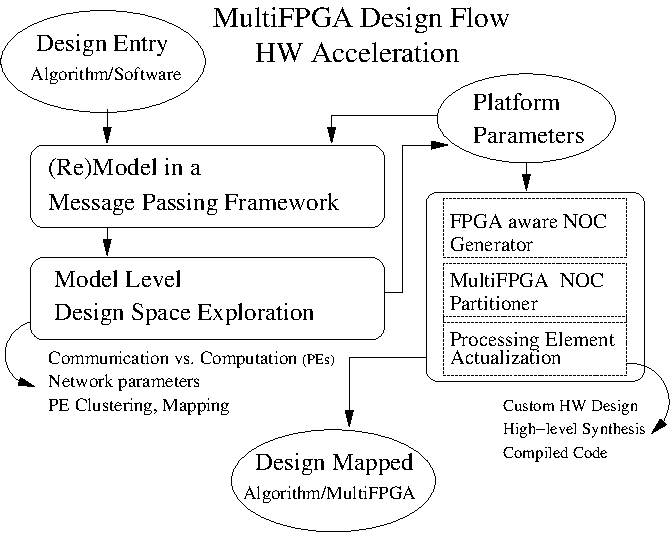
\includegraphics[scale=0.65]{xfig/hpcDesFlow.pdf}
\caption{Design flow applicable for Hardware Acceleration}
\label{fig:hpcDesFlow}
\end{figure}
Figure~\ref{fig:hpcDesFlow} outlines a design flow for multi-FPGA hardware acceleration.
The design entry is usually an application/algorithm that can benefit from hardware acceleration, scaling over multiple FPGAs. The next phase is to express/re-model the algorithm
in a framework of software threads---corresponding to processing elements in hardware---communicating in a message passing fashion.
%(which could be modeled with MPI~\cite{mpi-3.0} for instance). 
The target platform parameters such as the topology of choice, number of FPGAs could be selected to suit the model of the algorithm, with an awareness of constraints such as link-bandwidths, and resources.
% This modeling is done with an awareness of the platform generation parameters such as the topology of choice, link bandwidths, number of FPGAs and details; if necessary, the parameters could be changed if that suits the application. 
 
It is to be noted that the effort here is comparable to that of mapping to commodity accelerator architectures such as CUDA~\cite{CUDA:Programming-Guide}; only here, 
the broad parameters of the accelerator architecture, including scaling, are customizable by the designer. A software implementation of the model, for instance, could be done with  MPI~\cite{mpi-3.0}. The next optional step is a design 
space exploration at this model level to profile for the computation and communication traffic behaviors. The information at this stage could be used for processing element clustering (mapping to an FPGA) and partitioning (across FPGAs); 
the wealth of research on PE mapping~(e.g. \cite{1411933}) reported in the context of NoCs could be leveraged here. 

The next phase of the automation is hardware generation and has two steps: Processing element actualizations, and Network generation and partition. The network with the chosen parameters (topology, router configuration, etc.,) 
is generated by an FPGA architecture aware NoC generator,  which is followed by partitioning of the NoC across the available number of FPGAs. Actualizing the processing elements (PEs)---corresponding to the software threads 
of the message passing model---could be done via custom designed soft IPs or can be obtained through a High-level synthesis flow such as Vivado\cite{vivado}. A PE could even be a custom processor executing the corresponding cross-compiled code.
% After the FPGA architecture aware NoC generator, and the NOC partitioner across multiple FPGAs generate the platform as per specified parameters, the final step is that of actualizing the processing elements (corresponding to the software threads 
% of the message passing model). These PEs could be custom designed soft IPs or those obtained through a High-level synthesis flow~\cite{vivado}. A PE could even be a custom processor that would run the corresponding cross-compiled code.
%As a toy flow: we have developed a LLVM based (simple) C to ``Threads interacting over MPI'' generator with arbitrarily balanced partitioning and cross-compiling each thread again to custom lightweight processor, however, serious acceleration efforts may not expect automation at this level.

\subsection{ASIC prototyping}
At least at the modeling level (e.g.~\cite{ocpip}), there have been efforts (from both IP vendors and integrators) towards standardized IP/module interface in the context of Network-on-Chip based SoC integration. 
If~\cite{dally201321st} the component modules (processors, CODECS, MODEMS, etc.)  and subsystems (memory, IO) of the system use standard interfaces for communication over a packed-switched NoC, the 
multi-FPGA [rapid] prototyping of MPSoCs that integrate such components could be achieved using the proposed design automation. Even those MPSoC designs not so large as to require multiple FPGAs could still be effortlessly partitioned
across a multi-FPGA platform: this enables faster design to debug cycles owing to localization of bugs and partial reconfigation of specific FPGAs.

Also, unlike hardware acceleration which could potentially use arbitrarily large number of FPGAs, many ASIC [rapid] prototyping cases need less. And in this context,
% Also, ASIC [rapid] prototyping does not typically need as many FPGAs the hardware acceleration could use, which could potentially be arbitrarily large. And in this context,
 we note that the proposed scheme is particularly suitable for single-package multi-FPGA solutions such as Virtex 7 series FPGAs enabled by Stacked Silicon Integration~\cite{xilwp380}.

\section{Multi-FPGA Partitioning of Custom NoC}
\label{sec:mfpga_part}
\subsection{Problem}

While extending the NoC methodology for achieving communication between multiple FPGAs seems to be a compelling idea, there are multiple challenges which need to be addressed in this regard. We list down some of the important challenges here:
\begin{enumerate}
	\item \emph{First}, NoCs frequently use large port-width (consisting of few 10s of bits) for communication between interconnected routers, but the number of I/O pins on an FPGA is severely limited to meet this requirement. This concern is further aggravated in high radix topologies, where the NoC routers have high fan-out.
	\item \emph{Second}, the inter-FPGA interconnect delays are often high and also highly variable, especially when the different FPGAs are residing on separate boards. This makes it harder to achieve reliable communication using NoC.
	\item \emph{Third}, it is hard to have a common clock reference across multiple FPGAs without the use of Phase Locked Loops (PLLs) and synchronizers. This further complicates the design. Moreover, modules on different FPGAs could be optimized towards different operating speeds, in which case it may be suitable to operate them on different clock domains. This adds further complications to communicate in a synchronous manner.
\end{enumerate}

In order to resolve these challenges, we use asynchronous serial communication between the partitioned networks. This not only minimizes the requirement of a large number of parallel I/O pins for communication between partitioned networks, but also eliminates the need for a common clock reference. To this effect, our partitioning problem can be stated as: ``Given a set of interconnected routers and input/output ports, partition the network into disjoint subsets of routers, with each partition containing the specified set of routers, inter-connected in the same fashion with routers and the associated I/O ports within the partition, and insert and expose appropriate serial interface for interconnections across the partition." We require that the additional interfacing logic at network partitions be such that the application  modules using the network interface and the network routers themselves must remain oblivious to the partitioning. Figure~\ref{fig:part} provides an an example of NoC 
partitioning of four routers on two FPGAs, with communication between the FPGAs using a serializer/deserializer interface. 


\begin{figure}[t!]
\centering
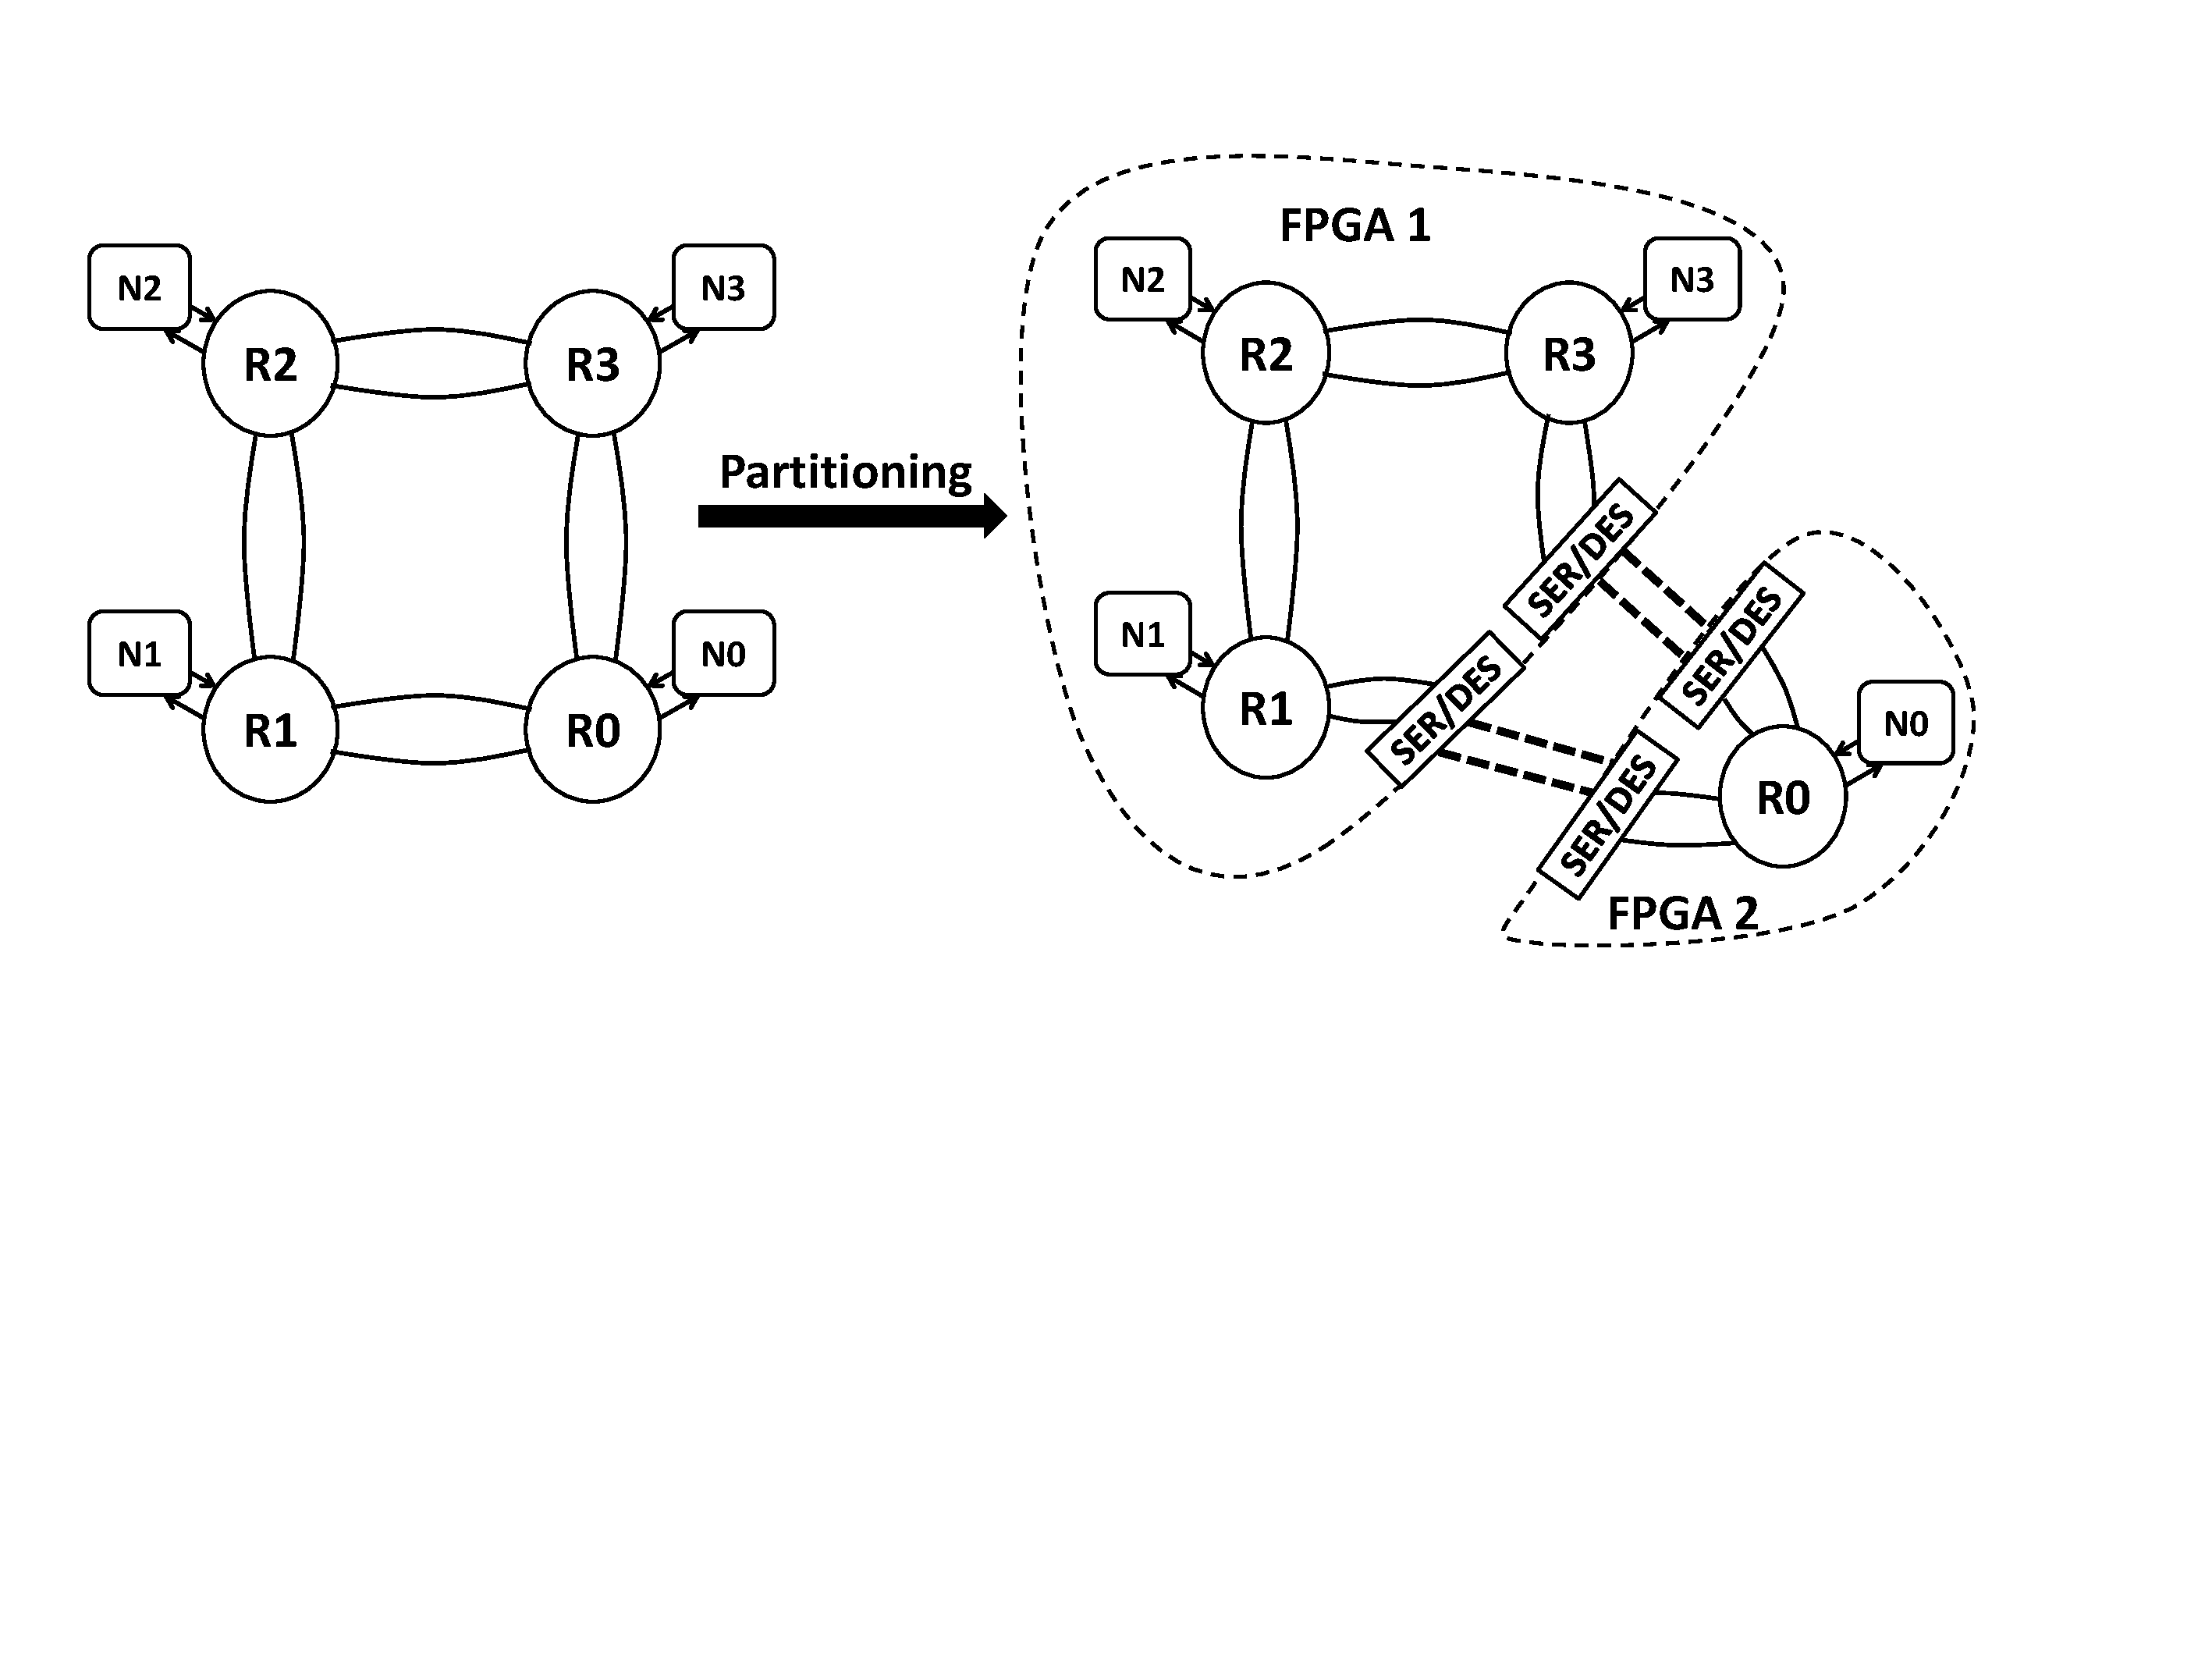
\includegraphics[scale=0.2]{figs/partitioning.pdf}
\caption{Example partitioning of an NoC with four routers on two FPGAs. The router R0 (along with its processing element N0) is mapped onto a separate FPGA. Communication between FPGAs takes place using serializer/deserializer (SER/DES) interface.}
\label{fig:part}
\end{figure}


%\begin{figure}[t!]
%\centering
%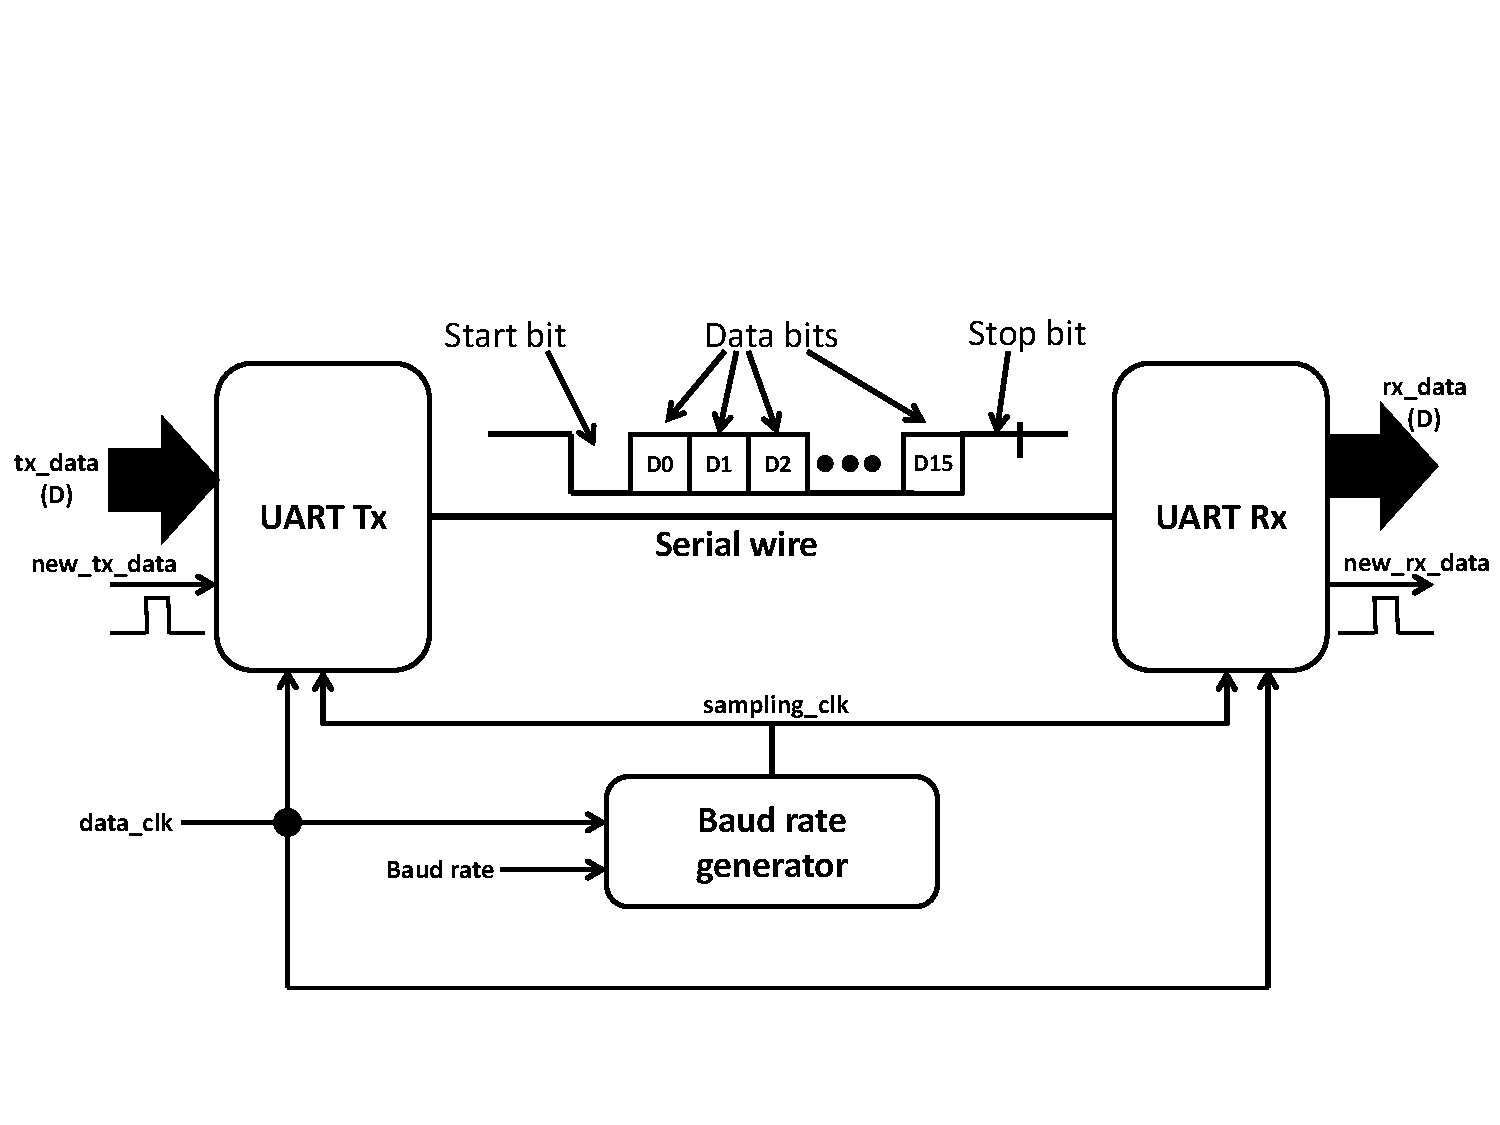
\includegraphics[scale=1, width=8cm]{figs/serial.pdf}
%\caption{Serial transmission using UART.}
%\label{fig:serial}
%\end{figure}


\subsection{Implementation Details}

Dally et. al~\cite{dally201321st} recently advocated for standard NoC generators for modularized designs to improve the design productivity. Separation of application development from the communication infrastructure having a standard interface improves the development time as well as the testing and verification costs. We use a freely available web-based synthesizable RTL generator for custom Network-on-Chip (NoC), named CONNECT(Configurable Network Creation Tool). CONNECT~\cite{papamichael2012connect} can be used for generating a NoC of arbitrary topology and supports a large variety of router and network configurations. Also, CONNECT incorporates a number of useful features fine-tuned for the FPGA platform, as opposed to the other popular NoC generators that are primarily intended for ASIC development.

As stated previously, we require asynchronous serial interface for across-the-FPGA communication. For this purpose, we use a variant of Universal Asynchronous Receiver/Transmitter (UART) protocol in which 16 bits (instead of 8 bits) are serially transmitted and received in a single frame. The UART transmitters and receivers contain shift registers operating nominally at the same frequency (typically much lower than the operating frequency of the hardware), known as the baud frequency, generated by a baud generator. This is also the sampling frequency for the receiver. In general, the data clocks at the transmitter and receiver side could be different and the sampling clock could be provided by the local baud generators, as long as the baud rate remains the same. 
%We have implemented separate modules for the baud generator and the UART transmitter and receiver. 



\begin{figure*}[htpb!]
\centering
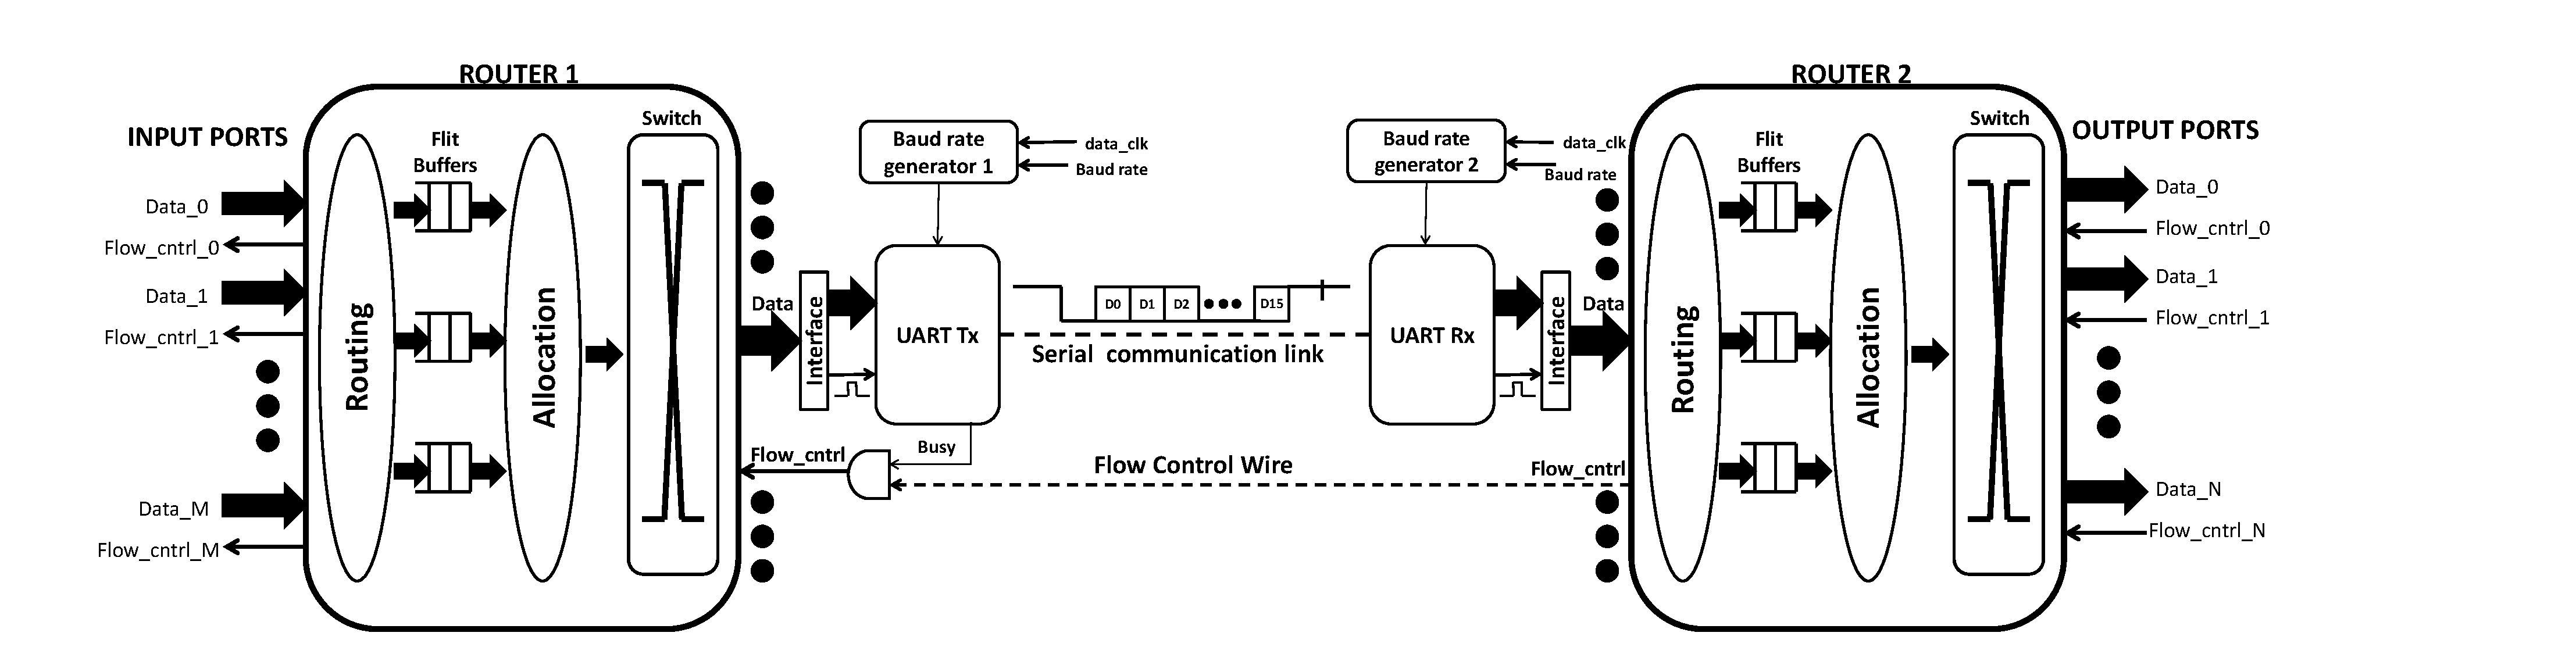
\includegraphics[scale=0.28]{figs/interface.pdf}
\caption{Communication between routers using UART. Dotted lines indicate the wires crossing the interface.}
\label{fig:interface}
\end{figure*}


Our script automatically partitions an input NoC into separate sub-networks which can be inter-connected via this serial interface. 

%This script is designed for partitioning NoCs generated using the CONNECT tool with the following parameters:
%\begin{itemize}
%	\item \textbf{Router Type:} Simple Input Queued (IQ)
%	\item \textbf{Flow Control Type:} Peek Flow Control
%	\item \textbf{Allocator:} Separable Input first Round-Robin
%\end{itemize}
Since flow control signals are also required to cross the FPGA partition along with the serial data links, we would like to minimize the number of flow control signals required in view of the limited I/O pin availability on a single FPGA. For this reason, we use peek flow control over credit based flow control. Peek flow control requires only a single bit signal per port for flow control. Additionally, peek flow control eliminates the need for maintaining registers for storing credits. We also do not use Virtual Channels (VCs) although it helps maximize network performance. This is also to minimize the FPGA pin count requirement, since flow control occurs on a per-VC basis. Also note that our approach can be easily integrated within the CONNECT NoC generator to directly generate partitioned sub-networks, with the input parameters provided in advance. 
 
 
We now describe the additional custom logic required to interface asynchronous serial communication using our UART modules with the CONNECT generated NoC in a manner that the rest of the modules remain unaffected. First, individual flits in CONNECT carry information about the destination address. This information also needs to be communicated to receiving routers over serial links along with the data bits. So, the data transfer port on the UART transmitter is connected to the lines corresponding to the destination bits and lowest significant bits of the outgoing flt data, such that the total size equals 16 bits (for sizes larger than this, the frame size must be further increased). Similarly, on the receiver side, the bits carrying the destination address to the receiving router are appropriately connected to the corresponding bits on the received data port of UART receiver. On the transmitter side, the representing a valid flit signal is connected to the input of the UART corresponding to the valid data signal to prompt the UART transmitter to start transmitting the incoming data. The upstream router does not assert its valid flit signal when the UART transmitter is busy or when the downstream router is not ready (through the incoming flow control signal indicating full buffer). Similarly, the UART receiver prompts the downstream router to receive incoming flit when the receiver has completely received the serially transmitted data frame. Figure~\ref{fig:interface} shows an example of two routers along with the additional UART circuitry. In practice, the SER/DES links\cite{athavale2005high} are to be implemented over the many (Multi Giga Bit Transiever) MGT links; this is a work in progress.


\subsection{Advantages}

The following is an enumeration of some advantages of the proposed approach.
\begin{itemize}
\item The approach enforces  \emph{modularity} and \emph{information hiding} in a multi-FPGA design, further improving design productivity and development time of multi-FPGA designs. 
The user-modules are oblivious to the NoC partitioning infrastructure, and the application developer is not required to be aware of details of serialization/deserialization details of the implementation.
\item Scales seemlessly with the number of partitions and modules.
\item The partitioning is flexible in terms of choice in topology and routing owing to CONNECT FPGA optimized NoC generator.
\item This NoC-based partitioning approach allows several modules operating at different clock speeds to effortlessly communicate with each other.%This is because the partitioned network uses asynchronous serial links instead of synchronous parallel wires to communicate with adjacent routers. 
In fact, our approach could be used in prototyping voltage-frequency islands for \emph{GALS}-based networks-on-chip onto FPGAs as described in~\cite{ogras2007voltage}. The authors have demonstrated 40\% energy savings using this approach on real video applications.
%\item When extended to use \emph{high-speed} interconnect technology, such as RapidIO~\cite{athavale2005high}, instead of UART links to achieve higher performance. This is a work in progress. 
%\item When the serialization/deserialization are implemented through the multi-gigabit transiever IO resources  (work in progress) 
\end{itemize}

% \begin{itemize}
% 
% 	\item This approach \emph{scales} seamlessly to a large number of modules and FPGA partitions. The application developer is not required to be aware of the details of the serialization/de-serialization modules used by the NoC. The user modules are also \emph{oblivious} to the NoC partitions and may continue to use the NoC in the same manner as without the partition. 
% 	\item The partitioning is flexible in terms of network \emph{topology} and \emph{routing}. Since the network is generated using CONNECT modules, it is also optimized for FPGA fabric.
% 	\item This NoC-based partitioning approach allows several modules operating at different clock speeds to effortlessly communicate with each other.%This is because the partitioned network uses asynchronous serial links instead of synchronous parallel wires to communicate with adjacent routers. 
% In fact, our approach could be used in prototyping voltage-frequency islands for \emph{GALS}-based networks-on-chip onto FPGAs as described in~\cite{ogras2007voltage}. The authors have demonstrated 40\% energy savings using this approach on real video applications.
% 	\item  Since the routers use serial links to communicate across different FPGA partitions, this approach minimizes the requirement of sparsely available \emph{I/O pins} on the FPGA. Use of peek flow control, instead of credit-based flow control, further helps in this regard.
% 	\item This approach enforces \emph{modularity} and \emph{information hiding} in a multi-FPGA design, further improving design productivity and development time of multi-FPGA designs.
% 	\item Our approach also allows for \emph{design-space exploration} (DSE) of NoCs over multiple-FPGAs. A network topology could have significant bearing on the overall performance and DSR would help strike the right balance between network cost and performance. 
% 	\item Our approach can be extended to use \emph{high-speed} interconnect technology, such as RapidIO~\cite{athavale2005high}, instead of UART links to achieve higher performance. This is a work in progress. 
% \end{itemize} 


\section{Case Study: Boolean Matrix Vector Multiplication}\label{sec:BMVM}
Boolean matrix vector multiplication (BMVM) has important applications in coding theory 
%~\cite{1216697},
and cryptanalysis
%~\cite{lenstra1990number} and image compression~\cite{swanson1996binary}
, among others. Several secure systems today rely on the computational intractability of factoring large
numbers~\cite{wiener1990cryptanalysis} and the Number Field Sieve (NFS) (Lenstra, \cite{lenstra1990number}) is perhaps the fastest known factorization algorithm.
Of the four major steps in NFS, \emph{Sieving} and \emph{Matrix Step} are considered to be the most time-consuming steps in the
NFS~\cite{anand2007factoring}. In particular, the Matrix Step involves finding linear dependencies
in a large boolean matrix. Block Wiedemann~\cite{coppersmith1994solving} algorithm is often used for
this purpose.  This translates to several Krylov sequence computations ($Av_{i}, A^{2}v_{i}, ... , A^{r}v_{i}$) involving a very large boolean matrix $A$ (dimensions in the range $10^6\to10^{11}$), and 
a large number of random boolean vectors $v_{i}$, with $i$ ranging from $1$ to $r$, where $r = 2D/K$. Here, $D$ is the column size of matrix $A$ and $K$ is known as the ``blocking
factor".

Our choice of BMVM as a case study has been influenced by a couple of factors, other than our research interest in accelerating iterative BMVM for NFS. First, our BMVM method is an instance of communication-intensive workload which benefits from the NoC design methodology. It's scalability is also ameliorated by our ability to partition network over multiple FPGAs. Secondly, we have encapsulated our hardware implementation in a software library using a standard CPU-FPGA integration tool which demonstrates how software development could benefit through multi-FPGA acceleration.
%Finally, accelerating iterative-BMVM for large matrices using FPGAs has been a long term research interest of our group for its Number Field Sieve application. 

\subsection{Previous work}
%Bernstein~\cite{bernstein2001circuits} 
%proposed a circuit-based implementation of the matrix-step NFS. 
Geiselmann et. al~\cite{geiselmann2003hardware} proposed a hardware
implementation of the "mesh routing" algorithm for matrix step in NFS using several interconnected 
ASICs. Bajracharya et. al~\cite{bajracharya2004reconfigurable} proposed an 
implementation of the above mesh routing circuit on a reconfigurable 
architecture. In mesh routing, a matrix $A$ of size $n\times n$, requires a mesh of 
size $m\times m$ nodes, where $m = \sqrt{n.h}$, $h$ being the maximum number of 
non-zero bits in any column of matrix $A$.  The $m\times m$ nodes are further divided 
into $D$ blocks, each of size $h\times h$, which are initialized with the input matrix 
$v$ and would produce the product vector $v'$ at the end of the algorithm. The 
$h$ nodes in a block $i$ are 
required to store the addresses (requiring $log(n)$ bits) of the non-zero bits 
in column $i$. For computing the product, each non-zero block would ``route" a 
message to target blocks corresponding to the $h$ addresses of that block, with 
each receiving block $i$, flipping its single-bit product value (initialized to 
0 before routing starts) corresponding to $i$-th bit in $v'$ on reception a 
message. ~\cite{bajracharya2004reconfigurable} have reported calculations indicating 1024-bit matrix step factorization possible in 27 days using 1024 FPGAs. Our method is better suited for handling ``dense" matrices and requires only sub-quadratic number of operations w.r.t. input matrix dimension by virtue of matrix pre-processing.
%{\red{TODO, mention quantitative information such as: \#FPGAs/ASICs vs. projected performance etc., to show the scale of the problem. 523 ASICs doing the 1024-bit factoring within a day.}}

\subsection{Method: Sub-quadratic algorithm to BMVM}
Our approach is based on the recently proposed
combinatorial algorithm for matrix vector multiplication by Ryan Willams~\cite{williams2007matrix}.
This approach involves a one-time pre-processing step on $A$, enabling a sub-quadratic time computation of BMVM.
% This approach involves a one-time pre-processing step on $A$ of $O(n^{2+\epsilon})$
% when $k = \epsilon . log(n)$), and thereafter enables BMVM in $O((n/k)^{2})$ on a $log(n)$-word RAM.
\begin{figure}[!htpb]
\centering
\subfloat[Tiling matrix $A$]{%
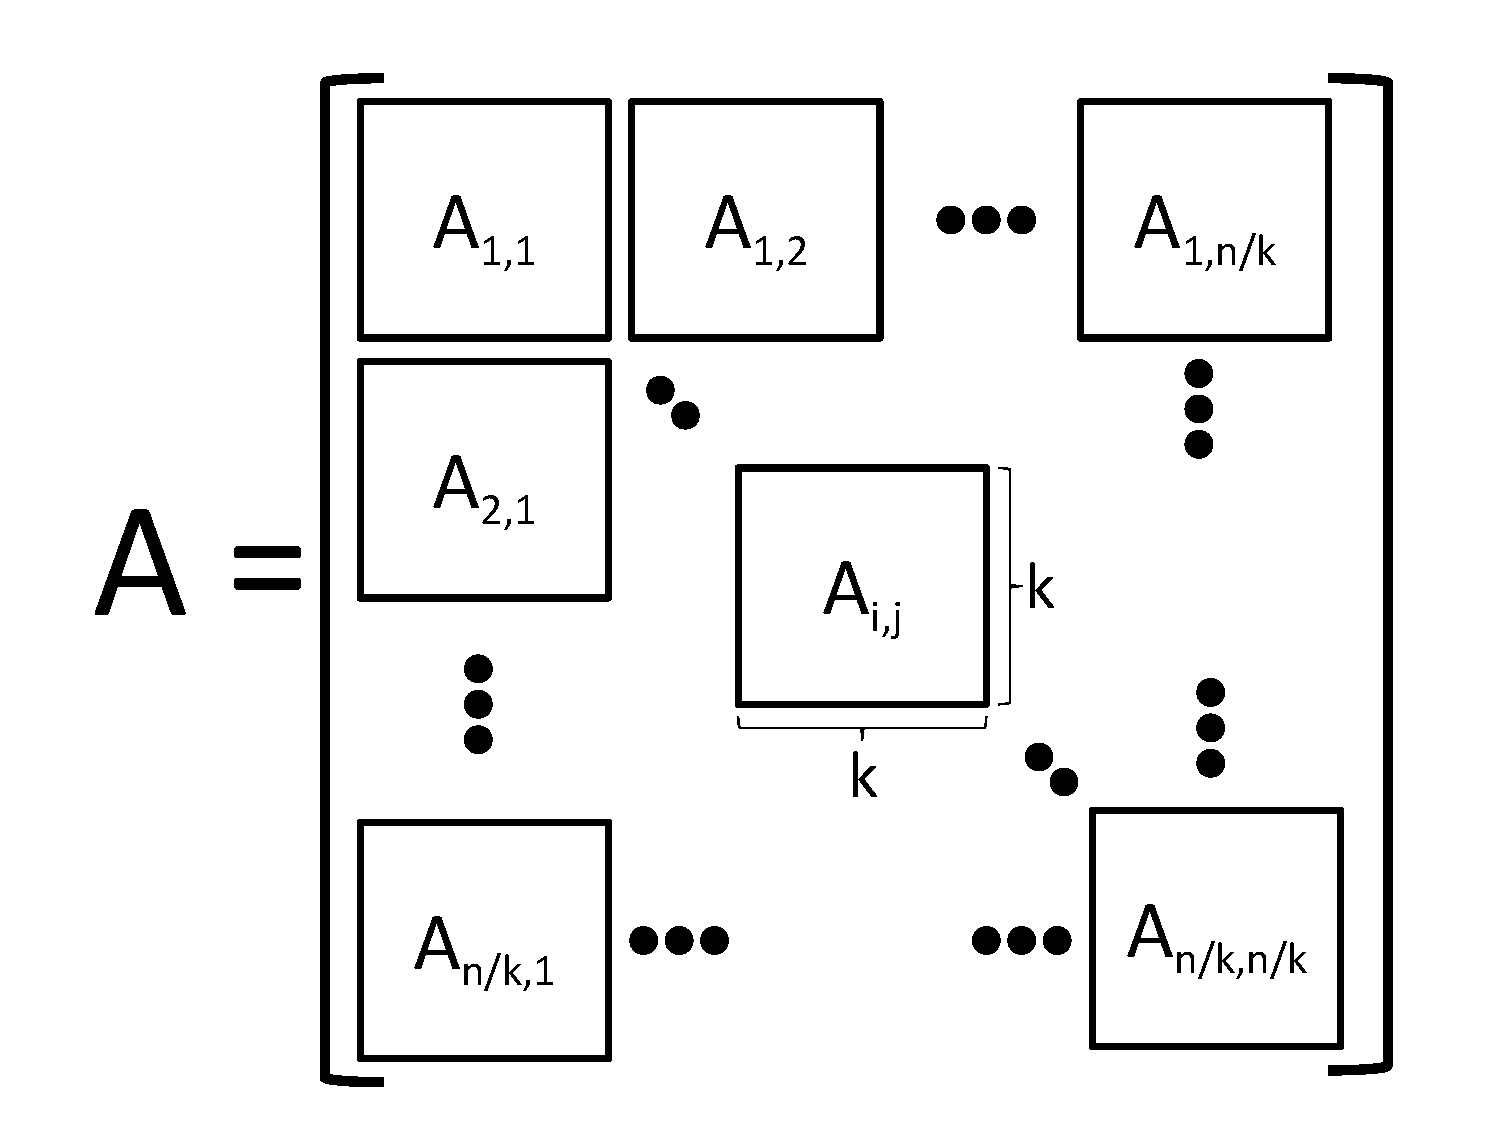
\includegraphics[scale=0.18]{figs/Pre-processing.pdf}
\label{fig:tiling}}
% \quad
\subfloat[Composition of the $LUT_i$]{%
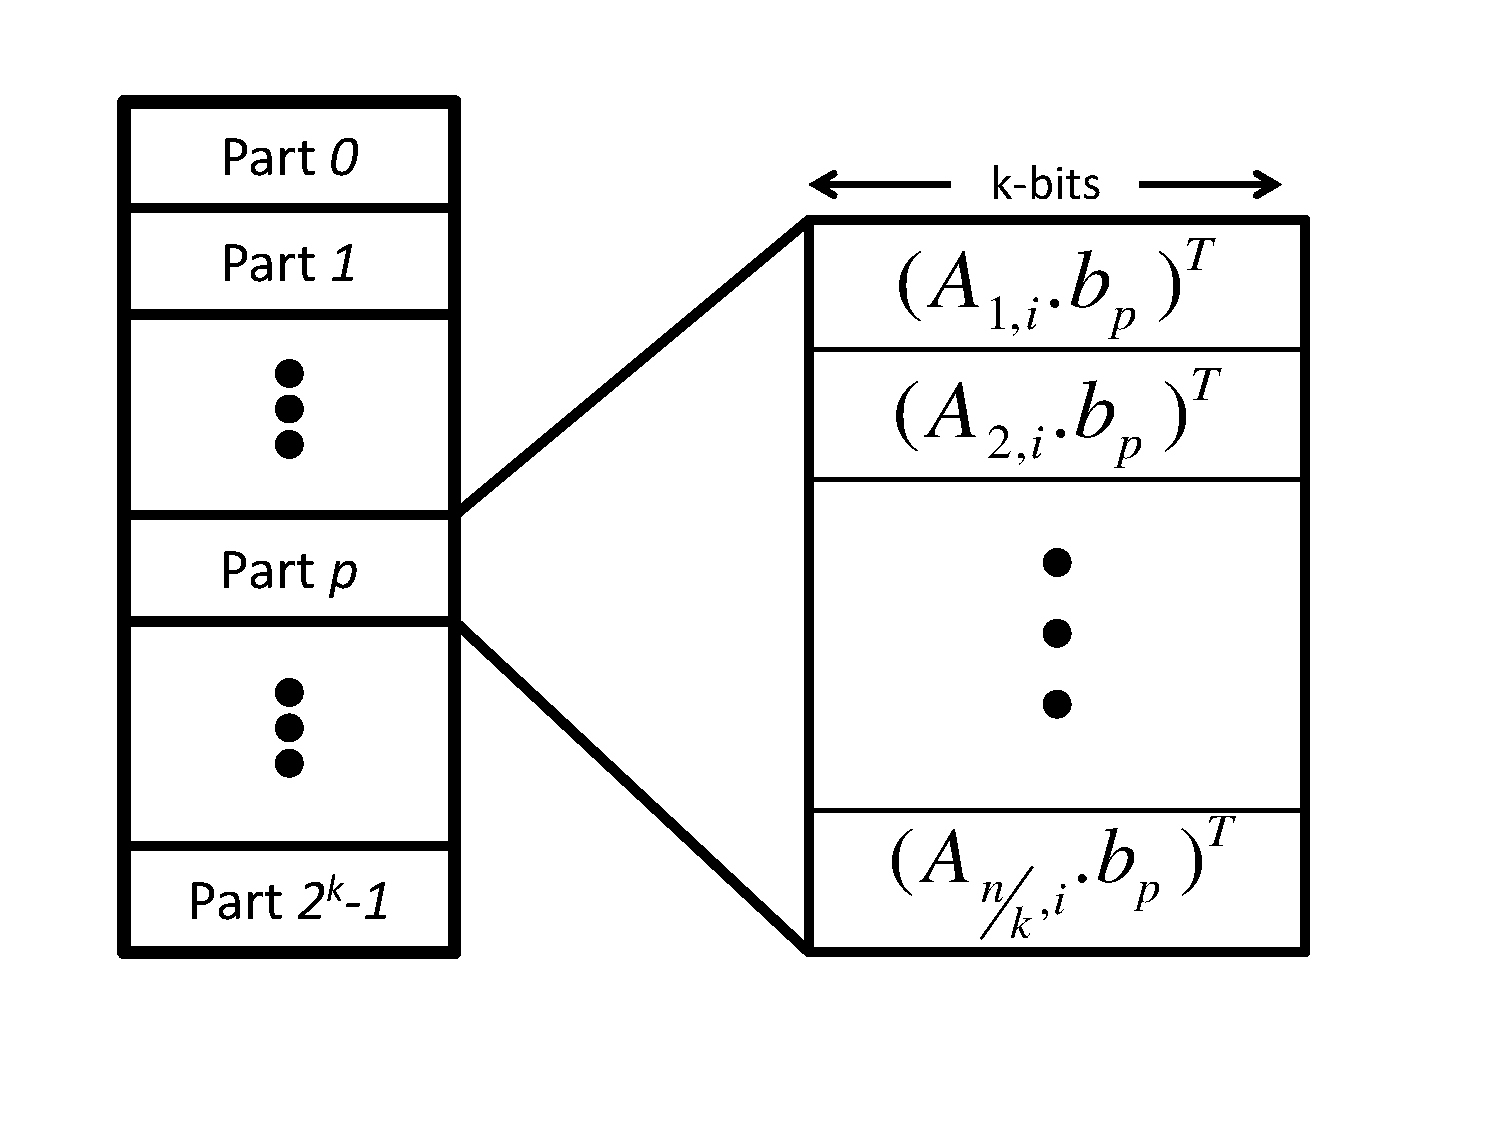
\includegraphics[scale=0.18]{figs/LUT.pdf}
\label{fig:lut_i}}
\caption{One-time pre-processing phase}
\label{fig:pre-process}
\end{figure}

The one-time pre-processing phase involves partitioning the matrix $A$ into tiles of dimensions $k\times k$ as in Figure~\ref{fig:tiling},
followed by construction of $n/k$ look-up tables $\{\, LUT_i \mid i: 1 \to n/k \,\}$ corresponding to each of the $n/k$ columns of the tiled $A$.
$LUT_i$ stores all possible linear combinations of columns of each $k\times k$ tile in the column $i$ of the tiled matrix $A$ (Figure~\ref{fig:tiling}).
There can be $2^k$ linear combinations of columns of each $k\times k$ tile, and there are $n/k$ such tiles in a column of A. 
Figure~\ref{fig:lut_i} shows the composition of $LUT_i$, which is partitioned into $2^k$ parts, each part storing $n/k$ $k-$bit words such that part$-p$ stores vectors
\{$A_{1,i}b_{p}, A_{2,i}b_{p}, ... , A_{n/k,i}b_{p}$\}, where $b_p$ is the $k$-bit vector corresponding to the partition index $p$. In short, the pre-processing step is equivalent to pre-computing and storing all possible products of
the tiles of matrix $A$ (ie., $A_{1,1}, A_{1,2} .. A_{n/k,n/k}$) with any $k$-bit vector.
 
The computing phase uses this pre-processed information to compute $Av$, for some vector $v$. Let $v$ be likewise partitioned into $n/k$ \emph{sub-vectors} ($v^T_1, v^T_2, .. , v^T_{n/k}$), and 
let $v' = Av = (v'^T_1, v'^T_2, .. , v'^T_{n/k})$. For illustration, let $LUT_i$, and $v^T_i$ be with processing node-$i$ (or thread-$i$). 
As $v'_i = A_{i,1}v_1\oplus A_{i,2}v_2 \oplus \ldots \oplus A_{i,n/k}v_n/k$, if each processing node-$i$ looks-up partition indexed by $v_i$ in $LUT_i$, and send each of the $n/k$ words stored
in this partition to the corresponding processing nodes, the result $v'_i$ at each processing node-$i$ is obtained by XOR-accumulating all the incoming $k$-bit messages.

In~\cite{williams2007matrix}, the authors have used $k = \epsilon log_2(n)$, with $\epsilon < 0.5$,
so that the multiplication can be carried out in $O(n^2/(\epsilon log(n))^2)$ on a $log(n)$-word
% RAM. The implications of choice of parameter $k$ are summarized in Table~\ref{tab:kchoice}.
 RAM. The implications of choice of parameter $k$ are summarized below.
% \begin{table}
\begin{center}
 \begin{tabular}{|r|l|}
 \hline
Word width of LUT & $k$ \\
Number of LUTs & $n/k$ \\
Size of each LUT (in words) & $2^k.(n/k)$ \\
Number of word operations required & $n^2/k^2$ \\  
\hline
 \end{tabular}
\end{center} 
%  \caption{Choice of $k$}
%  \label{tab:kchoice}
% \end{table}
% 
% It is observable that increasing the value of $k$ would reduce the computation time due to the
% reduced number of operations, but would, in turn, also increase the memory requirement (in LUTs) and
% the pre-processing time (occurring in $O(2^k.(n^2/k^2))$ ) exponentially. A careful selection of the
% parameter $k$ is thus required for achieving the right balance between the three. Also note that the
% extreme case when $k = n$ requires a single LUT storing $n$-bit product vectors corresponding to all
% possible $2^n$ combinations of input vector. Any multiplication would only require a single look-up
% into the corresponding entry. However, this is exponential in memory and pre-processing time and
% cannot be applied to matrices exceeding a few 10s of bits in size.
% 

\subsection{Implementation Details}~\label{sec:Impl}
The pre-processing stage is one-time and has been done
as described above, in software.
%\subsubsection{TARGET--NoC-driven multi-FPGA}
The three components involved in this mapping are: the processing node architecture, the network infrastructure and the FPGAs.
As our processing nodes need to contain LUTs, which are efficiently mapped to the onchip Block RAMs available in abundance on modern FPGAs (Virtex 6, for instance, has large number of 
$36Kb$ BRAMs totalling  upto $38 Mb$). Depending on the problem parameters ($n$ and $k$), not all processing nodes can be mapped to a single FPGA.
As per our earlier discussion, we map all the $n/k$ processing elements across all the FPGAs in our NoC-driven multi-FPGA platform. 
It is important to  ensure that while multiple such messages may simultaneously attempt to update a 
particular product sub-vector $v'_i$, the updates are appropriately serialized 
to maintain correctness. Since only one flit can be injected and ejected in a 
single cycle in the NoC, this constraint is automatically ensured. Our 
implementation supports the following ``Network and Router Options" for NoC 
generated using CONNECT (topology and number of endpoints is user-specified):
% \begin{table}	
\begin{center}
 \begin{tabular}{|r|l|}
 \hline
	{Router Type} & Simple Input Queued (IQ)\\
	{Flow Control Type}& Peek Flow Control\\
	{Flit Data Width}& 16\\
	{Flit Buffer Depth}& 8\\
	{Allocator}& Separable Input first Round-Robin\\
\hline
 \end{tabular}
\end{center}

%\red{Folding, and other details}
Since number of sub-vectors can be very large ($n/k$), we also implement ``folding", such that a single processing element is handles multiple sub-vectors and is provided with a single coalesced look-up table corresponding to the input sub-vectors. The extent of this folding is referred to as the ``folding factor" $f$. Figure~\ref{fig:pe} shows a single processing element, and figure~\ref{fig:mult_top} shows the top module consisting of several such processing elements connected by a CONNECT generated NoC, which can also be partitioned over multiple FPGAs. Our final step is to integrate this setup with software to make it usable as a FPGA-accelerated software library. We achieve this using RIFFA 2.0~\cite{jacobsen2013riffa}. Figure~\ref{fig:riffa} shows the overall framework. Our implementation also supports iterative BMVM to compute $Av, A^{2}v, ... , A^{r}v$, with number of iterations $r$ communicated by the software endpoint to the FPGA along with the input vector $v$. 

\begin{figure}[t!]
\centering
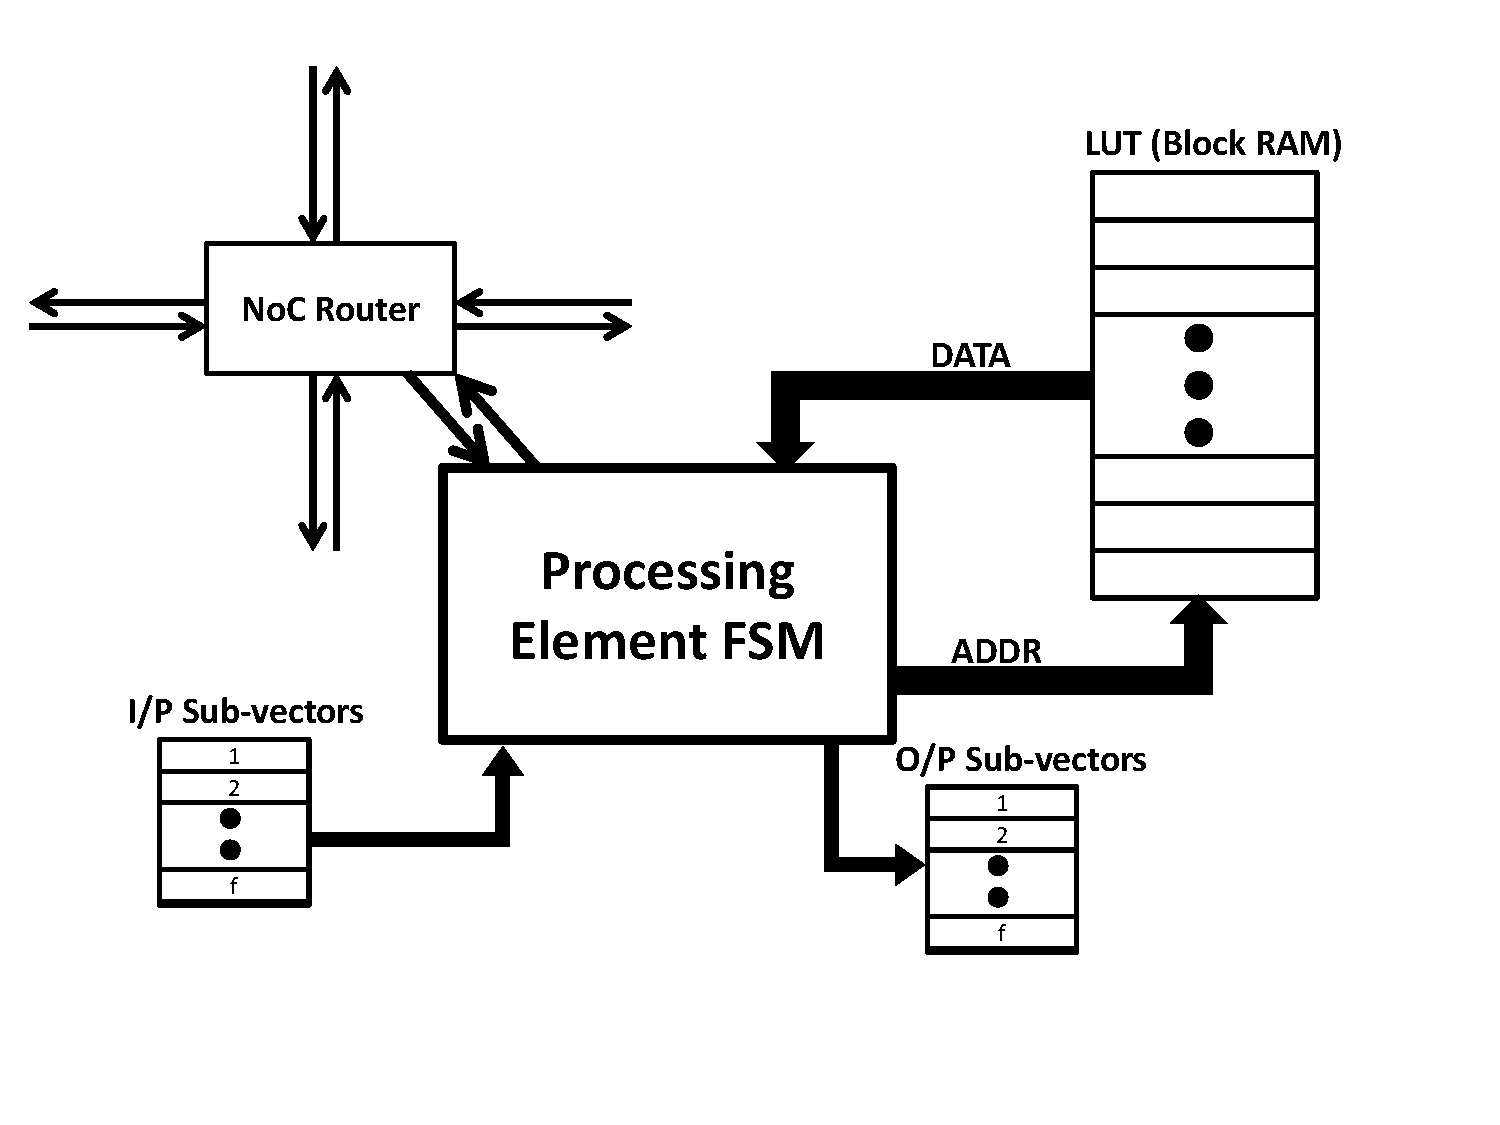
\includegraphics[scale=0.3]{figs/processing_element.pdf}
\caption{Processing element.}
\label{fig:pe}
\end{figure}

\begin{figure}[t!]
\centering
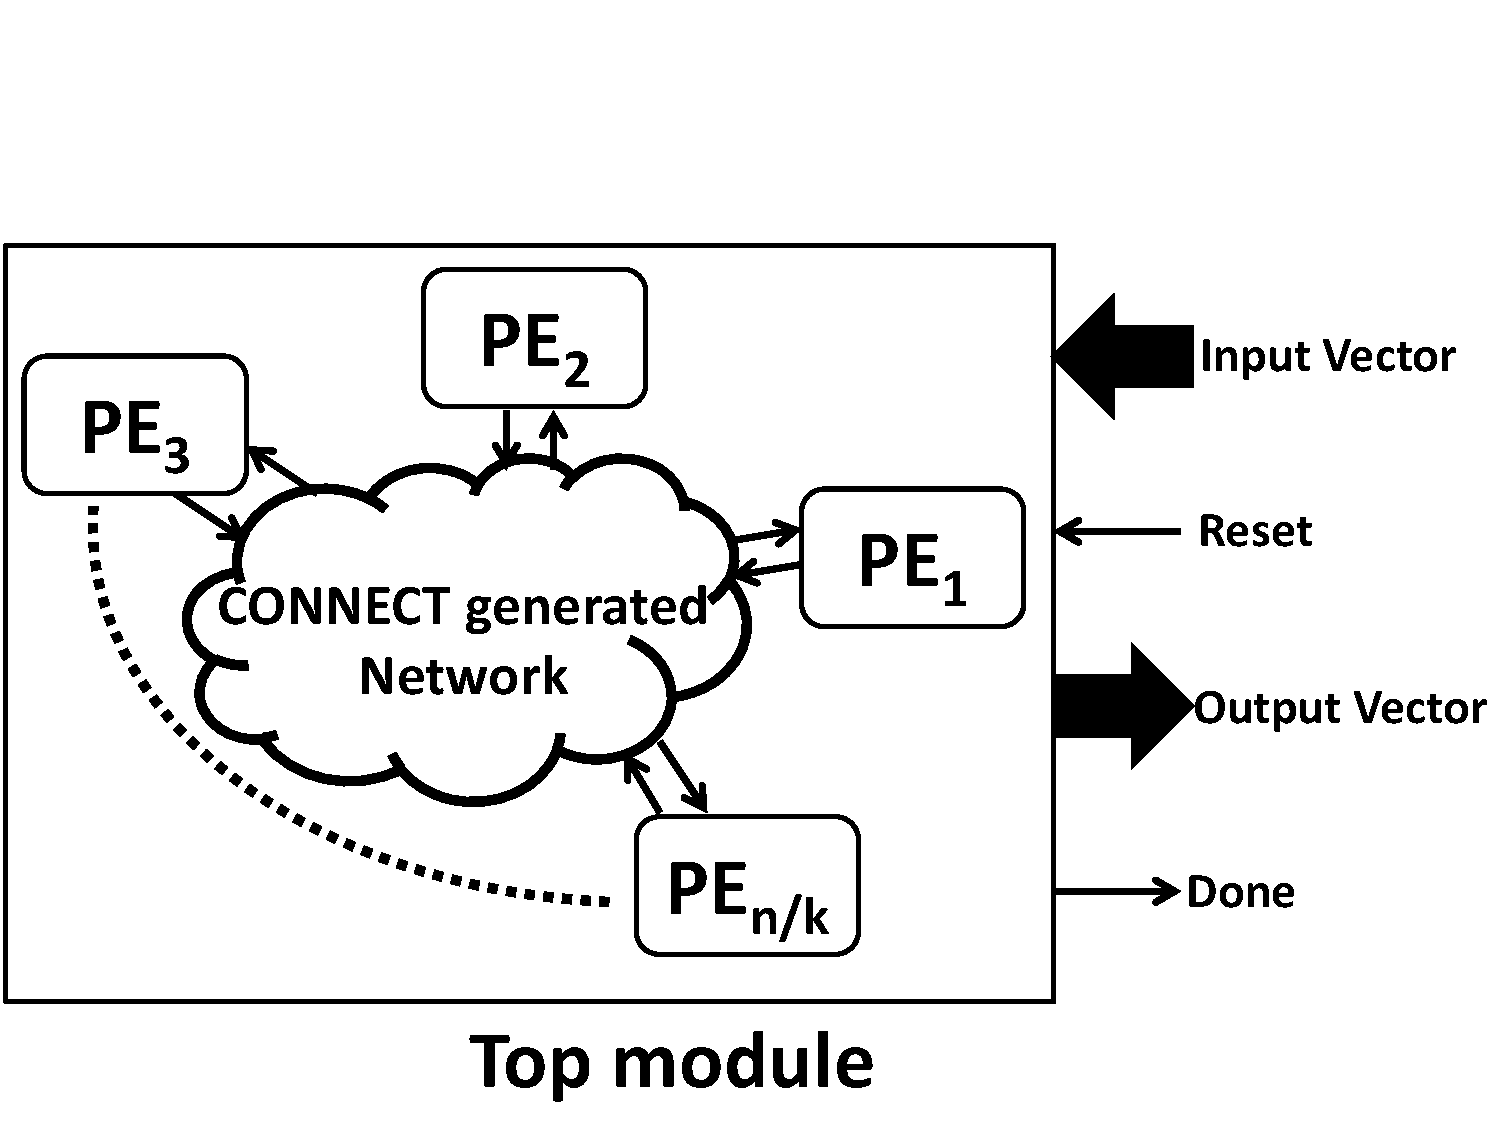
\includegraphics[scale=0.3]{figs/mult_top.pdf}
\caption{Top module for Boolean Matrix Vector Multiplication (BMVM).}
\label{fig:mult_top}
\end{figure}

\begin{figure}[t!]
\centering
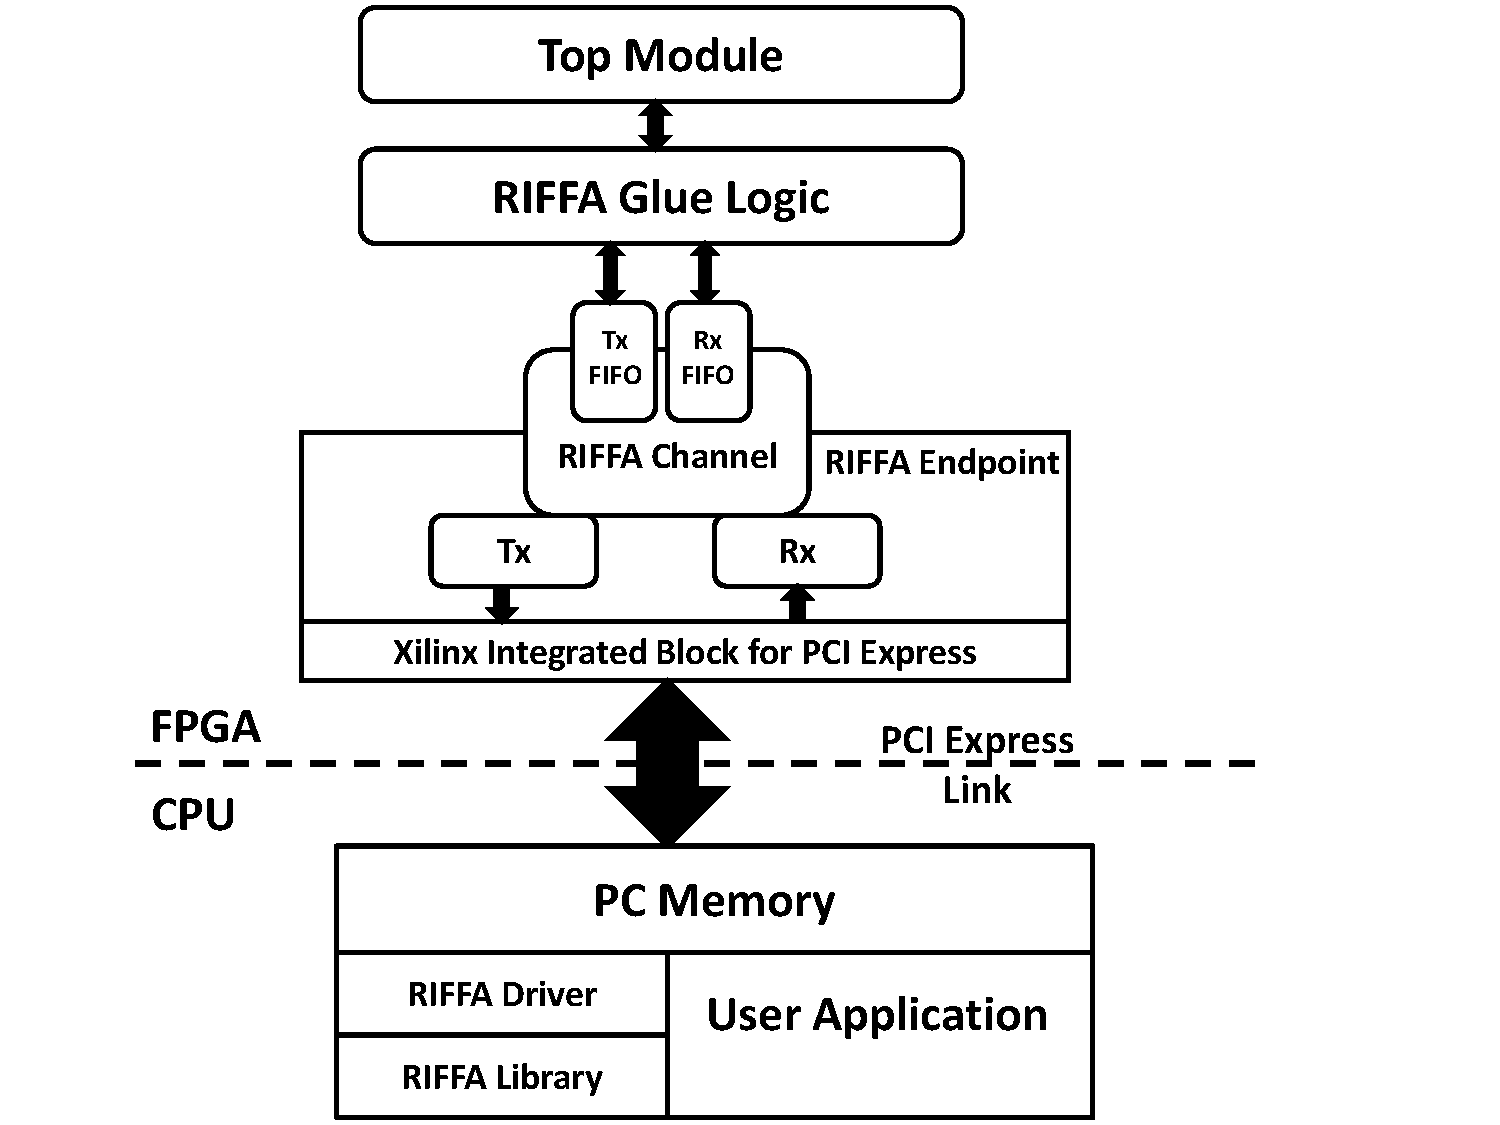
\includegraphics[scale=0.34]{figs/riffa.pdf}
\caption{BMVM framework with RIFFAa.}
\label{fig:riffa}
\end{figure}

\section{Experimental Results}

% SW
% configuration
% Setup

For experimental evaluation, we implemented our hardware on Xilinx Virtex 6 ML605 XC6VLX240T-1FFG1156 Evaluation Board using Xilinx 14.3 ISE, with software endpoint running on a 1.6 GHz Intel i7-2600 processor. We have also implemented a multi-threaded equivalent software implementation of the described algorithm using the \emph{pthread} library, with each thread corresponding to one precessing element in its hardware equivalent. Concurrent updates of multiple threads are serialized using \emph{locks} and \emph{barriers} are used in between successive iterations. Our multi-threaded software BMVM was evaluated on a 1.2 GHz six core (dual thread) Intel Xeon E5-2620 processor (Model 45, 15360 KB cache) and was used as a baseline for comparison. Our hardware modules were made to operate at 100MHz clock, with partitioned networks using a UART interface with baud rate of 115200 bits/second. We evaluate our implementation on following two configurations:

\noindent \textbf{Configuration 1: $n = 64, k = 8, f = 2$}\\

\begin{table*}[!htpb]
  \centering
	\begin{tabular}{| l | l | l | l | l | l |}
	\hline
	Iterations & \multicolumn{3}{c}{Time (in msec)} \vline & \multicolumn{2}{c}{Speedup (Norm. to Software)} \vline \\
%\cmidrule(r){1-2}
	 \cline{2-6}
 	& Software & Mesh & Partitioned Mesh & Mesh & Partitioned Mesh \\
 \hline
 
	 1 & 0.32 & 0.052 & 1.48 & 6.15 & 0.22  \\
	 10 & 1.1 & 0.052 & 14.14 & 21.15 & 0.078 \\
	 100 & 5.2 & 0.087 & 140.3 & 59.8 & 0.037 \\
	 1000 & 44.2 & 0.58 & 1402.8 & 76.2 & 0.031 \\
	%\midrule
\hline

%\bottomrule
\end{tabular}
\caption{Comparative results for configuration 1 (average over 100 experiments).}
\label{table_c1}
\end{table*}

\noindent \textbf{Configuration 2: $n = 1024, k = 4, f = 4$}\\

\begin{table*}[!htpb]
  \centering
	\begin{tabular}{| l | l | l | l | l | l | l | l | l | l |}
	\hline
	Iterations & \multicolumn{5}{c}{Time (in msec)} \vline & \multicolumn{4}{c}{Speedup (Norm. to Software)} \vline \\
%\cmidrule(r){1-2}
	 \cline{2-10}
 	& Software & Ring & Mesh & Torus & Fat\_tree & Ring & Mesh & Torus & 	Fat tree\\
 \hline
 
	 1 & 4.0 & 0.205 & 0.075 & 0.060 & 0.052 & 19.5 & 53.3 & 66.7 &  76.9 \\
	 10 & 22.9 & 1.67 & 0.412 & 0.299 & 0.275 & 13.71 & 55.58 & 76.6 & 83.3 \\
	 100 & 204.3& 16.15 & 3.64 & 2.83 & 2.33 & 12.7 & 56.12 & 72.2 & 87.7 \\
	 1000 & 2025.4 & 160.51 & 35.60 & 28.09 & 22.69 & 12.6 & 56.9 & 72.1 & 89.3 \\
	%\midrule
\hline

%\bottomrule
\end{tabular}
\caption{Comparative results for configuration 2 (average over 100 experiments).}
\label{table_c2}
\end{table*}

Configuration 1 requires four processing elements (threads) for a input matrix of size $64 \times 64$. As a proof of concept, we partitioned the input $2 \times 2$ mesh on two separate FPGAs. We have reported the execution time (including roundtrip over RIFFA interface) for partitioned as well as unpartitioned mesh. As can be observed from the result tables, the partitioned mesh results in a slowdown due to the slow speed UART bottleneck. We are working on using faster interconnection links to get speedup results comparable to single cycle unpartitioned mesh.

Configuration 2 requires 64 processing elements for a matrix of size $1024 \times 1024$. We have evaluated the results for four network topologies implemented on a single FPGA with single cycle hop between adjacent routers, which depict a clear correlation between network cost and performance (the cost increases moving from ring to mesh to torus to fat tree but performance also improves accordingly). When number of iterations are low (1-10), the overheads in terms of host processor - FPGA communication time in hardware and thread \emph{creation/join} time in software, are a dominant component of the overall execution time. For larger iterations (100-1000), the actual computation times dominate and the total execution time increases nearly linearly with number of multiplication iterations.



\section{Related work}
\label{sec:relwork}

Network-on-Chip has been a topic of immense interest in the last decade. A rich 
body of work exists on several themes concerning NoC, such as application-specific topology, 
routing, micro-architecture, power, placement, verification, among others. 
Multi-FPGA partitioning for prototyping of large designs dates back to the 
pre-NoC era, when the FPGA was a lot more resource constrained. Ouaiss et. 
al~\cite{ouaiss1998integrated} developed "SPARCS", a synthesis and partitioning 
tool for multi-FPGA systems, with shared memory or direct channel communication 
between partitioned tasks. Roy-Neogi et. al~\cite{roy1995multiple} suggested a 
genetic algorithm based partitioning method for multiple FPGAs within resource 
and timing constraints. Papamichael et. al~\cite{papamichael2012connect} 
developed an automated NoC generator tool tailor-made for FPGAs. Liu et. 
al~\cite{liu2010building} and Mostefaoui et. al~\cite{4669212}have developed a multi-FPGA emulation framework, with 
MGT transceivers for communication. However, the system only ``mimics" NoC, and 
does not implement it on FPGA.

Our work bears most similarity with Fleming et. al~\cite{Fleming:2012:LLE:2145694.2145725}, who were perhaps the first to propose a packetized communication mechanism for multiple FPGAs having automated network partitioning. However, their work is more narrowly focused around automated partitioning for a class of latency-insensitive hardware designs that conform to a specific model of computation. They also do not use serial communication between FPGAs, which is why their pin count requirement would be large. Stepniewska et. al~\cite{stepniewska2010network} have also worked on a similar idea using high speed serial I/O on FPGA.



% \blue{
% \subsection{Relevant focus areas for FSP}
% \begin{itemize}
% \item Design automation for multi-FPGA and heterogeneous systems.
%  \item Overlays: FPGA-aware CONNECT\cite{papamichael2012connect}  + NoC + Processors?
%  \item Mapping approaches and tools for heterogeneous FPGAs.
%  \item HLS. High-level compilation and languages, design automation tools that 
% raise the abstraction level when designing for (heterogeneous) FPGAs and 
% reconfigurable systems and standardized target platforms. 
%  \item Application case studies.
% \end{itemize}
% }
\section{Conclusion and Future work}
\label{sec:conclusion}

Multi-FPGA partitioning has historically been considered a tough challenge, owing to the difficulty in contriving communication interfaces between separate FPGAs. Our automated approach to Network-on-Chip partitioning, based on a standard, freely available NoC generator, not only placates this challenge, but also extends the pervasive NoC design methodology to the multi-FPGA scenario. Our Boolean Matrix Vector Multiplication (BMVM) application demonstrates the utility of our partitioning technique for scalability and prototyping of large hardware designs. Our FPGA implementation of BMVM can achieve orders of speedup compared to its software counterpart, even at modest clock frequencies, if provisioned with high-speed interconnects. Our preliminary investigations make a case for NoC-based FPGA designs for hardware acceleration and prototyping. This work opens up avenues for research and lays a strong foundation for further exploration of some pertinent ideas. Our ongoing work aims to extend our methodology to use faster interconnect technologies for inter-FPGA communication and calibrating our boolean matrix vector multiplication algorithm to handle large and sparse matrices.

\bibliographystyle{ieeetr}
% argument is your BibTeX string definitions and bibliography database(s)
\bibliography{IEEEabrv,ref}

% that's all folks
\end{document}
